\documentclass[12pt,a4paper]{article}
\setlength{\parindent}{0pt}
% Paquetes
\usepackage[utf8]{inputenc}
\usepackage[spanish]{babel}
\usepackage{amsmath,amssymb,amsthm}
\usepackage{graphicx}
\usepackage{booktabs}
\usepackage{hyperref}
\usepackage{geometry}
\usepackage{fancyhdr}
\usepackage{enumitem}
\usepackage{caption}
\usepackage{subcaption}
\usepackage{float}
\usepackage[style=ieee, backend=biber]{biblatex}
\addbibresource{Bibliografia.bib}
\usepackage{multirow}
\usepackage{array}
\usepackage{xcolor}
\usepackage{colortbl}
\usepackage{tikz}
\usepackage{pgfplots}
\usepackage{listings}
\usepackage{breakurl}
\pgfplotsset{compat=1.18}

\geometry{margin=2.5cm}
\hypersetup{
    colorlinks=true,
    linkcolor=blue,
    urlcolor=blue,
    citecolor=blue
}

% Configuración de listings para código
\lstset{
    basicstyle=\ttfamily\small,
    breaklines=true,
    frame=single,
    backgroundcolor=\color{gray!5},
    numbers=left,
    numbersep=5pt,
    numberstyle=\tiny\color{gray},
    keywordstyle=\color{blue},
    commentstyle=\color{green!40!black},
    stringstyle=\color{red}
}

% Título
\title{\textbf{Modelo de Ising para Criminalidad en Bogotá}\\[0.3cm]

\vspace{2cm}

       \large Proyecto Final - Mecánica Estadística\\[0.3cm]
       \normalsize Programa Académico de Física\\[0.3cm]
       \normalsize Universidad Distrital Francisco José de Caldas}
\author{Juan David Chaparro Rojas\\
Miguel Angel Ramos Higuera\\
Samuel Homez Caicedo
}
\date{\today}

\begin{document}

\maketitle

\begin{center}

\includegraphics[width=0.3\textwidth]{Escudo_UD.png}
\end{center}

\thispagestyle{empty}
\newpage

% ============================================================================
% RESUMEN
% ============================================================================
\begin{abstract}\noindent
Este proyecto aplica el modelo de Ising de la física estadística para modelar la dinámica criminal en Bogotá D.C., utilizando \textbf{1,068,340 llamadas} a la línea de emergencias 123 (2015-2026) y \textbf{4 fuentes de datos abiertos} (estratificación socioeconómica, deserción escolar, Comandos de Atención Inmediata y pobreza). \\
\noindent
El modelo de Ising, originalmente diseñado para describir transiciones de fase en materiales magnéticos, se adapta aquí para modelar la \textbf{propagación del crimen} entre Unidades de Planeamiento Zonal (UPZ) vecinas. Cada UPZ se trata como un ``espín'' que puede estar en estado activo ($+1$, alta criminalidad) o inactivo ($-1$, baja criminalidad), y la interacción entre UPZs vecinas captura el efecto de contagio espacial.

Los resultados principales muestran que:
\begin{itemize}
    \item El modelo base (con efectos fijos por UPZ) alcanza un \textbf{AUC = 0.971} en predicción de hotspots criminales
    \item El contagio espacial existe pero es moderado ($J = 0.4336$), explicando solo el 59\% de la predictibilidad
    \item Los campos locales $h_i$ (vulnerabilidad intrínseca) son el factor dominante
    \item El \textbf{92.5\%} de la variación en $h_i$ entre UPZs puede explicarse mediante variables observables
    \item La deserción escolar es el predictor más robusto de criminalidad ($r = 0.54$)
    \item El sistema se encuentra en \textbf{fase desordenada} ($T_{\text{eff}} = 1.29 > T_{\text{crit}} = 0.89$)
\end{itemize}

\textbf{Palabras clave:} modelo de Ising, sociofísica, criminalidad, Bogotá, datos abiertos, contagio espacial, mecánica estadística.
\end{abstract}

\newpage
\tableofcontents
\newpage

% ============================================================================
% 1. INTRODUCCIÓN
% ============================================================================
\section{Introducción}

\subsection{Motivación}
La criminalidad urbana es uno de los problemas más apremiantes en las ciudades latinoamericanas. Bogotá D.C., con más de 8 millones de habitantes, presenta patrones criminales complejos que varían tanto en el espacio como en el tiempo. Comprender estos patrones no solo requiere identificar \textit{dónde} ocurre el crimen, sino también \textit{cómo se propaga} entre zonas vecinas y \textit{qué factores estructurales} lo determinan.

Los enfoques tradicionales en criminología (teoría de la desorganización social, teoría de la oportunidad, \textit{hotspot policing}) han proporcionado marcos valiosos, pero raramente incorporan la \textbf{dinámica temporal} y la \textbf{interacción espacial} de manera simultánea. La física estadística ofrece herramientas matemáticas precisamente diseñadas para modelar sistemas con muchas partículas interactuantes.

\subsection{Objetivos}
\begin{enumerate}[label=\alph*)]
    \item Adaptar el modelo de Ising para modelar la dinámica criminal en Bogotá
    \item Estimar el parámetro de contagio espacial ($J$) y los campos locales ($h_i$) a partir de datos reales
    \item Incorporar variables socioeconómicas para explicar los campos locales
    \item Evaluar la capacidad predictiva del modelo mediante validación cruzada temporal
    \item Derivar implicaciones de política pública basadas en los resultados
\end{enumerate}

% ============================================================================
% 2. MARCO TEÓRICO
% ============================================================================
\section{Marco Teórico}

\subsection{El Modelo de Ising en Física Estadística}

El modelo de Ising, propuesto por Wilhelm Lenz en 1920 y resuelto en una dimensión por Ernst Ising en 1925~\cite{ising1925}, es el modelo canónico para estudiar transiciones de fase en sistemas magnéticos. Consiste en un conjunto de $N$ partículas (espines) dispuestas en los nodos de una red, cada una de las cuales puede encontrarse en dos estados: $s_i = +1$ (espín ``arriba'') o $s_i = -1$ (espín ``abajo''). La energía de una configuración particular $\{s\} = (s_1, s_2, \ldots, s_N)$ está dada por el Hamiltoniano:

\begin{equation}\label{eq:hamiltoniano}
H(\{s\}) = -J \sum_{\langle i,j \rangle} s_i s_j - \sum_{i=1}^{N} h_i s_i
\end{equation}

donde $\langle i,j \rangle$ denota pares de espines vecinos en la red, $J$ es la constante de acoplamiento que determina la fuerza y naturaleza de la interacción entre vecinos, y $h_i$ es un campo magnético externo que actúa sobre el sitio $i$. Cuando $J > 0$, el sistema es ferromagnético: la energía se minimiza cuando los espines vecinos están alineados ($s_i s_j = +1$), favoreciendo configuraciones ordenadas con todos los espines apuntando en la misma dirección.

En equilibrio termodinámico a temperatura $T$, la probabilidad de encontrar el sistema en una configuración $\{s\}$ sigue la distribución de Boltzmann~\cite{onsager1944}:

\begin{equation}\label{eq:boltzmann}
P(\{s\}) = \frac{1}{Z} \exp\left(-\frac{H(\{s\})}{k_B T}\right)
\end{equation}

donde $k_B$ es la constante de Boltzmann y $Z = \sum_{\{s\}} \exp(-H/k_B T)$ es la función de partición, que normaliza la distribución. La temperatura $T$ controla el balance entre orden (favorecido por la interacción $J$) y desorden (favorecido por la agitación térmica). A temperaturas bajas ($T < T_c$, donde $T_c$ es la temperatura crítica), el sistema se encuentra en una fase ordenada con magnetización no nula; a temperaturas altas ($T > T_c$), la agitación térmica destruye el orden y el sistema transita a una fase desordenada o paramagnética.

Tres observables macroscópicos caracterizan el comportamiento del sistema:

\begin{itemize}
    \item \textbf{Magnetización}: $M = \frac{1}{N}\sum_{i=1}^{N} s_i$. Mide el orden global: $M \approx \pm 1$ indica alineamiento casi total (fase ordenada), mientras que $M \approx 0$ indica desorden (fase paramagnética).
    \item \textbf{Correlación espacial}: $C = \frac{1}{N_{\text{edges}}}\sum_{\langle i,j \rangle} s_i s_j$. Promedio del producto de espines sobre todos los pares vecinos; cuantifica el grado de alineamiento local.
    \item \textbf{Susceptibilidad magnética}: $\chi = N \cdot \text{Var}(M)$. Mide la sensibilidad del sistema a perturbaciones externas: alcanza un máximo en la vecindad de $T_c$, donde el sistema es más susceptible a pequeños cambios en el campo externo.
\end{itemize}

\subsection{Analogía Sociofísica}

La adaptación del modelo de Ising al contexto de la criminalidad urbana~\cite{castellano2009,prieto2020} establece una correspondencia directa entre los conceptos de la física estadística y los fenómenos criminológicos, resumida en la Tabla~\ref{tab:analogia}.

\begin{table}[H]
\centering
\caption{Analogía entre el modelo de Ising y la criminalidad urbana}
\label{tab:analogia}
\begin{tabular}{@{}p{2.5cm}p{1.8cm}p{9.5cm}@{}}
\toprule
\textbf{Concepto Físico} & \textbf{Símbolo} & \textbf{Interpretación Criminológica} \\
\midrule
Espín & $s_i = \pm 1$ & UPZ con alta ($+1$) o baja ($-1$) actividad criminal en un mes \\
Interacción & $J$ & Fuerza del contagio criminal entre UPZs que comparten frontera \\
Campo externo & $h_i$ & Vulnerabilidad intrínseca de cada UPZ (factores estructurales: pobreza, educación, infraestructura) \\
Temperatura & $T$ & Nivel de impredictibilidad del sistema (factores no modelados) \\
Magnetización & $M$ & Proporción global de UPZs con alta actividad criminal \\
Susceptibilidad & $\chi$ & Sensibilidad de la ciudad a intervenciones o shocks externos \\
Correlación & $C$ & Grado de clustering espacial del crimen entre UPZs vecinas \\
\bottomrule
\end{tabular}
\end{table}

El principio físico fundamental se traduce directamente: si $J > 0$, el sistema tiende a alinear espines vecinos (ferromagnetismo), lo que en el contexto criminal significa que una UPZ con alta actividad delictiva \textbf{aumenta la probabilidad} de que sus vecinas también presenten alta actividad en el período siguiente. La temperatura $T$ captura todos los factores no modelados explícitamente que introducen aleatoriedad en el sistema: eventos impredecibles, factores externos no medidos, o fluctuaciones intrínsecas de la actividad criminal.

\subsection{Dinámica de Glauber y Predicción Temporal}

El modelo de Ising en equilibrio (Ecuaciones~\ref{eq:hamiltoniano} y~\ref{eq:boltzmann}) describe probabilidades de configuraciones estáticas, pero no proporciona un mecanismo para modelar la evolución temporal del sistema. Para aplicaciones predictivas, es necesario dotar al modelo de una dinámica que especifique cómo transita el sistema de un estado al siguiente.

La solución estándar en física estadística es la \textbf{dinámica de Glauber} (Glauber, 1963), un proceso estocástico Markoviano diseñado para que la distribución estacionaria del sistema converja exactamente a la distribución de Boltzmann en equilibrio. En esta dinámica, los espines se actualizan secuencialmente: en cada paso de tiempo discreto se selecciona un espín al azar y se determina su nuevo estado con base en el campo local que experimenta, definido como la suma de las interacciones con sus vecinos más cualquier campo externo. La probabilidad de transición es:

\begin{align}\label{eq:glauber}
    P(s_i \to +1) &= \frac{\exp\left(+\beta\left[J\sum_{j \in \partial i} s_j + h_i\right]\right)}
{\exp\left(+\beta\left[J\sum_{j \in \partial i} s_j + h_i\right]\right) + 
 \exp\left(-\beta\left[J\sum_{j \in \partial i} s_j + h_i\right]\right)}\\
&= \sigma\!\left(2\beta\Bigl[J\sum_{j \in \partial i} s_j + h_i\Bigr]\right)
\end{align}

donde $\beta = 1/(k_B T)$, $\partial i$ denota el conjunto de vecinos del sitio $i$ en la red, y $\sigma(x) = 1/(1+e^{-x})$ es la función sigmoide (logística). La Ecuación~\ref{eq:glauber} muestra que la probabilidad de que un espín adopte el valor $+1$ depende exclusivamente del campo local que siente en ese instante, comprimido al intervalo $[0,1]$ por la función sigmoide.

Para nuestro modelo criminal, adoptamos esta dinámica con dos adaptaciones. Primero, interpretamos cada paso de la dinámica como un intervalo de \textbf{un mes}, de modo que el estado en $t+1$ depende del estado observado en $t$. Segundo, absorbemos el factor $2\beta$ dentro de los parámetros $J$ y $h_i$, puesto que la temperatura efectiva $T_{\text{eff}}$ del sistema se estimará posteriormente mediante un procedimiento independiente de simulación Monte Carlo (Sección~\ref{sec:termodinamica}). Esto conduce a la \textbf{ecuación fundamental de predicción} del modelo:

\begin{equation}\label{eq:dinamico}
\boxed{P\left(s_i(t+1) = +1 \;\middle|\; \mathbf{s}(t)\right) = 
       \sigma\!\left(J \sum_{j \in \partial i} s_j(t) + h_i\right)}
\end{equation}

La Ecuación~\ref{eq:dinamico} tiene una interpretación criminológica directa. La probabilidad de que una UPZ presente alta actividad criminal en el mes siguiente depende de dos contribuciones aditivas dentro del argumento de la sigmoide:

\begin{enumerate}[label=\alph*)]
    \item \textbf{Contagio espacial}: $J \sum_{j \in \partial i} s_j(t)$. Si los vecinos de la UPZ $i$ están mayoritariamente activos ($s_j = +1$), la suma es positiva y este término \textit{aumenta} la probabilidad de activación. Si están mayoritariamente inactivos ($s_j = -1$), el término es negativo y \textit{reduce} dicha probabilidad. La magnitud de $J$ determina la fuerza de este efecto de contagio.
    
    \item \textbf{Vulnerabilidad intrínseca}: $h_i$. Es un sesgo fijo característico de cada UPZ que captura todos los factores estructurales persistentes que afectan su propensión criminal (pobreza, deserción escolar, infraestructura urbana, presencia institucional), independientemente del estado de sus vecinos. Un valor $h_i > 0$ predispone a la UPZ a la actividad criminal; un valor $h_i < 0$ indica resistencia estructural al crimen.
\end{enumerate}

La función sigmoide actúa como mecanismo de saturación: comprime cualquier valor real del campo local total al intervalo $[0,1]$, garantizando una probabilidad bien definida. Es monótona creciente, con $\sigma(0) = 0.5$ (máxima incertidumbre), $\sigma(x) \to 1$ cuando $x \to +\infty$ (activación casi segura), y $\sigma(x) \to 0$ cuando $x \to -\infty$ (inactivación casi segura).

\textbf{Propiedad Markoviana.} La dinámica de Glauber define un proceso de Markov de primer orden: el estado en $t+1$ depende únicamente del estado en $t$, no de la historia completa del sistema. Formalmente:
\begin{equation}
P\left(\mathbf{s}(t+1) \mid \mathbf{s}(t), \mathbf{s}(t-1), \ldots, \mathbf{s}(0)\right) = 
P\left(\mathbf{s}(t+1) \mid \mathbf{s}(t)\right)
\end{equation}
Esta hipótesis es verificable empíricamente: si agregar rezagos temporales adicionales ($t-1$, $t-2$) como predictores no mejora significativamente el rendimiento del modelo, la propiedad Markoviana se sostiene. En las pruebas realizadas sobre los datos de Bogotá, el estado en $t$ captura la práctica totalidad de la información relevante para predecir $t+1$.

\textbf{Interpretación como regresión logística.} Una ventaja metodológica decisiva de la Ecuación~\ref{eq:dinamico} es que puede estimarse mediante \textbf{regresión logística estándar}. El log-odds de activación es lineal en los parámetros:
\begin{equation}\label{eq:logit}
\text{logit}\left[P(s_i(t+1) = +1)\right] = \ln\left(\frac{P}{1-P}\right) = J \sum_{j \in \partial i} s_j(t) + h_i
\end{equation}
Esto permite utilizar el amplio arsenal de herramientas de machine learning para la estimación (máxima verosimilitud con regularización L2 mediante \texttt{LogisticRegression} de scikit-learn), la inferencia estadística (errores estándar y $p$-valores mediante \texttt{Logit} de statsmodels) y la validación predictiva (validación cruzada temporal, curvas ROC). La física estadística proporciona el marco teórico y la interpretación de los parámetros; la ciencia de datos proporciona las herramientas de estimación y validación.

\subsection{Modelo Sociofísico Enriquecido}

El modelo de la Ecuación~\ref{eq:dinamico} asume que tanto el contagio $J$ como la vulnerabilidad $h_i$ son constantes universales. Sin embargo, es razonable esperar que la fuerza del contagio y la propensión criminal varíen sistemáticamente con las características socioeconómicas de cada UPZ. Para incorporar esta heterogeneidad de manera interpretable, extendemos el modelo permitiendo que ambos parámetros dependan de un vector de $K$ covariables observables $\mathbf{X}_i = (X_{i1}, X_{i2}, \ldots, X_{iK})$:

\begin{equation}\label{eq:sociofisico}
P(s_i=+1 \mid \mathbf{s}, \mathbf{X}) = \sigma\!\left(J_i(\mathbf{X}) \sum_{j \in \partial i} s_j + h_i(\mathbf{X})\right)
\end{equation}

donde la dependencia funcional se modela como lineal en las covariables:

\begin{align}
J_i &= \beta_0 + \sum_{k=1}^{K} \beta_k X_{ik} \label{eq:J_modulado} \\
h_i &= \alpha_0 + \sum_{k=1}^{K} \alpha_k X_{ik} \label{eq:h_explicado}
\end{align}

Esta formulación, que denominamos \textbf{modelo de Ising sociofísico}, tiene cuatro ventajas fundamentales sobre el modelo base con efectos fijos:

\begin{enumerate}[label=\alph*)]
    \item \textbf{Interpretabilidad}: Los coeficientes $\beta_k$ y $\alpha_k$ tienen significado criminológico directo. Un valor $\beta_k > 0$ indica que la variable $X_k$ \textit{amplifica} el contagio criminal (la UPZ es más ``permeable'' a la influencia de sus vecinos cuando $X_k$ es alto), mientras que $\beta_k < 0$ indica que $X_k$ \textit{bloquea} el contagio. Análogamente, $\alpha_k > 0$ ($\alpha_k < 0$) indica que $X_k$ \textit{aumenta} (\textit{reduce}) la propensión criminal intrínseca.
    
    \item \textbf{Accionabilidad}: Al expresar $J_i$ y $h_i$ como funciones de variables observables y potencialmente modificables mediante política pública (como la deserción escolar o la presencia policial), el modelo permite \textit{simular} el efecto de intervenciones antes de implementarlas.
    
    \item \textbf{Parsimonia}: Mientras que el modelo base requiere estimar $N + 1$ parámetros (un $h_i$ por cada UPZ más un $J$ global), el modelo sociofísico utiliza $2(K+1)$ parámetros. Con $K = 7$ covariables, esto representa 16 parámetros, una reducción de casi un orden de magnitud respecto a los 112 del modelo base.
    
    \item \textbf{Generalizabilidad}: Los parámetros $\beta_k$ y $\alpha_k$ capturan relaciones estructurales entre covariables y criminalidad que, en principio, son transferibles a otras ciudades con características similares, mientras que los efectos fijos $h_i$ son específicos de cada UPZ y no generalizables.
\end{enumerate}

% ============================================================================
% 3. DATOS Y METODOLOGÍA
% ============================================================================
\section{Datos y Metodología}

\subsection{Fuentes de Datos}

\begin{table}[H]
\centering
\caption{Fuentes de datos utilizadas}
\label{tab:fuentes}
\begin{tabular}{@{}lll@{}}
\toprule
\textbf{Fuente} & \textbf{Registros} & \textbf{Variables} \\
\midrule
Llamadas Línea 123 (2015-2026) & 1,068,340 & Tipo de incidente, UPZ, fecha \\
Estratificación (Manzanas) & 39,150 & Estrato socioeconómico \\
Deserción Escolar (UPZ) & 118 & Tasas por género y grado \\
CAIs & 154 & Ubicación de comandos policiales \\
Shapefile UPZ & 113 & Geometría, área, perímetro \\
\bottomrule
\end{tabular}
\end{table}

\subsection{Construcción de Espines}

Para cada UPZ $i$ y cada mes $t$, los espines se definen mediante umbrales basados en percentiles de la distribución histórica:

\begin{equation}\label{eq:espines}
s_i(t) = \begin{cases}
+1 & \text{si } \text{incidentes}_i(t) > P_{70}^{(i)} \\
-1 & \text{si } \text{incidentes}_i(t) < P_{30}^{(i)} \\
0  & \text{en otro caso}
\end{cases}
\end{equation}

Esto produce una matriz de $135 \text{ meses} \times 124 \text{ UPZs}$. La red de vecinos (frontera geográfica compartida) conecta 111 UPZs mediante 302 aristas (grado promedio $\approx 5.4$).

\subsection{Observables del Sistema Real}

De la matriz de espines calculamos: $M_{\text{obs}} = -0.0673$ (ligeramente más UPZs inactivas), $C_{\text{obs}} = 0.1210$ (correlación espacial positiva y significativa, $p < 0.001$), y $\chi_{\text{obs}} = 2.78$ (susceptibilidad no significativa, $p = 1.000$).

% ============================================================================
% 4. IMPLEMENTACIÓN COMPUTACIONAL
% ============================================================================
\section{Implementación Computacional}

\subsection{Librerías Utilizadas}

El proyecto se implementó en \textbf{Python 3.12}, utilizando las siguientes librerías especializadas. A continuación se describe cada una y su rol específico en la construcción del modelo.

\subsubsection{Pandas (\texttt{pandas})}

\textbf{Versión:} 2.2.0\\
\textbf{Propósito:} Manipulación y análisis de datos tabulares.\\
\textbf{Uso en el proyecto:} 
\begin{itemize}
    \item Carga del archivo CSV de 1,068,340 registros de llamadas al 123 mediante \texttt{pd.read\_csv()}, manejando diferentes codificaciones (latin1, utf-8) y delimitadores.
    \item Agregación de incidentes por UPZ y mes usando \texttt{groupby()} sobre las columnas \texttt{COD\_UPZ}, \texttt{ANIO\_NUM} y \texttt{MES\_NUM}.
    \item Construcción de la matriz de espines mediante \texttt{pivot\_table()}, transformando datos longitudinales a formato panel (meses $\times$ UPZs).
    \item Cálculo de umbrales dinámicos con \texttt{quantile(0.70, axis=0)} y \texttt{quantile(0.30, axis=0)} para cada UPZ.
    \item Preparación del dataset de entrenamiento con rezagos temporales ($t$ y $t+1$) para la regresión logística.
\end{itemize}

\subsubsection{NumPy (\texttt{numpy})}

\textbf{Versión:} 1.26.0\\
\textbf{Propósito:} Computación numérica eficiente con arreglos multidimensionales.\\
\textbf{Uso en el proyecto:}
\begin{itemize}
    \item Operaciones vectorizadas sobre la matriz de espines para calcular observables macroscópicos: $M = \texttt{S\_vals.mean(axis=1)}$, $C = 0.5 \cdot \texttt{np.sum((S\_vals @ adj) * S\_vals, axis=1)}$.
    \item Construcción de la matriz de adyacencia $\texttt{adj}$ de dimensiones $N \times N$ con tipo de dato \texttt{np.int8} para minimizar uso de memoria.
    \item Generación de números aleatorios (\texttt{np.random.rand}, \texttt{np.random.choice}) para el algoritmo de Metropolis y las pruebas de permutación.
    \item Cálculo de la función sigmoide para la probabilidad de activación: $\sigma(x) = 1/(1 + \texttt{np.exp}(-x))$.
    \item Operaciones de álgebra lineal para la simulación termodinámica: $\texttt{spins @ adj\_matrix @ spins}$.
\end{itemize}

\subsubsection{GeoPandas (\texttt{geopandas})}

\textbf{Versión:} 1.0.0\\
\textbf{Propósito:} Extensión de Pandas para datos geoespaciales, permitiendo trabajar con geometrías (puntos, polígonos) y realizar operaciones espaciales.\\
\textbf{Uso en el proyecto:}
\begin{itemize}
    \item Carga del shapefile de UPZs (\texttt{TAprobacionNOfUPZ\_2023.shp}) con \texttt{gpd.read\_file()}.
    \item Carga de datos abiertos geoespaciales: manzanas de estratificación (\texttt{ManzanaEstratificacion.shp}), deserción escolar (\texttt{TDesercionOfUPZ.shp}) y CAIs (\texttt{ComandoAtencionInmediata.shp}).
    \item Construcción de la red de vecinos mediante \texttt{geometry.touches()}, que identifica pares de UPZs que comparten frontera.
    \item Asignación espacial de manzanas y CAIs a UPZs mediante \texttt{gpd.sjoin()} con predicado \texttt{'intersects'} o \texttt{'within'}.
    \item Cálculo de áreas de UPZ (\texttt{geometry.area}) para normalizar la densidad de CAIs.
    \item Rotación y transformación de coordenadas con \texttt{affinity.rotate()} para la visualización.
    \item Exportación del dataset enriquecido a GeoJSON con \texttt{to\_file()}.
\end{itemize}

\subsubsection{Scikit-learn (\texttt{sklearn})}

\textbf{Versión:} 1.5.0\\
\textbf{Propósito:} Librería principal de machine learning con implementaciones eficientes de algoritmos de clasificación, regresión y validación.\\
\textbf{Uso en el proyecto:}
\begin{itemize}
    \item \texttt{LogisticRegression} (con penalización \texttt{l2} y solucionador \texttt{lbfgs}): estimación de los tres modelos de Ising (puro, base con dummies, y sociofísico). El parámetro \texttt{C} controla la fuerza de regularización.
    \item \texttt{roc\_auc\_score} y \texttt{roc\_curve}: evaluación del rendimiento predictivo mediante el área bajo la curva ROC.
    \item \texttt{confusion\_matrix}: construcción de la matriz de confusión para el modelo sociofísico.
    \item \texttt{precision\_recall\_curve}: análisis del trade-off entre precisión y sensibilidad.
    \item \texttt{calibration\_curve}: verificación de la calibración probabilística del modelo (diagrama de confiabilidad).
    \item \texttt{TimeSeriesSplit} (con \texttt{n\_splits=5}): validación cruzada temporal que respeta el orden cronológico de los datos.
    \item \texttt{learning\_curve}: análisis de la evolución del rendimiento con el tamaño del conjunto de entrenamiento.
    \item \texttt{RandomForestRegressor} (con \texttt{n\_estimators=300}): modelo no lineal para explicar $h_i$ en función de covariables.
    \item \texttt{permutation\_importance}: estimación de la importancia de cada variable mediante la disminución en $R^2$ al permutar sus valores.
    \item \texttt{StandardScaler}: normalización de variables para los índices compuestos.
    \item \texttt{PCA}: reducción de dimensionalidad para construir índices de cobertura educativa.
\end{itemize}

\subsubsection{Statsmodels (\texttt{statsmodels})}

\textbf{Versión:} 0.14.0\\
\textbf{Propósito:} Modelos estadísticos con inferencia formal (pruebas de hipótesis, intervalos de confianza).\\
\textbf{Uso en el proyecto:}
\begin{itemize}
    \item \texttt{Logit} (regresión logística con \texttt{sm.Logit}): estimación del modelo base con inferencia estadística completa, reportando coeficientes, errores estándar, valores $z$ y $p$-valores.
    \item \texttt{OLS} (mínimos cuadrados ordinarios con \texttt{sm.OLS}): regresión de $h_i$ sobre covariables socioeconómicas para cuantificar el poder explicativo ($R^2$) de los factores estructurales.
    \item Obtención de estadísticos de ajuste: log-verosimilitud (\texttt{llf}), criterio de información bayesiano (\texttt{bic}), pseudo-$R^2$ de McFadden (\texttt{prsquared}).
\end{itemize}

\subsubsection{SciPy (\texttt{scipy})}

\textbf{Versión:} 1.13.0\\
\textbf{Propósito:} Algoritmos de optimización y funciones estadísticas.\\
\textbf{Uso en el proyecto:}
\begin{itemize}
    \item \texttt{minimize\_scalar}: calibración de $J$ por máxima verosimilitud, encontrando el valor que minimiza la función de log-verosimilitud negativa en el intervalo $[0, 2]$.
    \item \texttt{pearsonr}: cálculo de la correlación de Pearson entre cada covariable y $h_i$, con su correspondiente $p$-valor para prueba de hipótesis bilateral.
    \item \texttt{minimize} (con método \texttt{L-BFGS-B}): optimización multivariada para el modelo con campo uniforme $h_0$.
\end{itemize}

\subsubsection{Matplotlib (\texttt{matplotlib})}

\textbf{Versión:} 3.9.0\\
\textbf{Propósito:} Visualización científica y generación de gráficas de alta calidad.\\
\textbf{Uso en el proyecto:}
\begin{itemize}
    \item \texttt{pyplot} y \texttt{GridSpec}: construcción de figuras multi-panel para diagnóstico del modelo.
    \item \texttt{ListedColormap}: creación de mapas de color personalizados para visualizar espines (rojo = $-1$, azul = $+1$).
    \item \texttt{FuncAnimation} + \texttt{PillowWriter}: generación de la animación GIF de propagación criminal (40 frames, 1 fps) usando el algoritmo de Metropolis.
    \item Mapas coropléticos de Bogotá usando GeoPandas + Matplotlib para visualizar $h_i$, deserción, estrato y CAIs.
\end{itemize}

\subsection{Arquitectura del Pipeline de Datos}

El flujo de procesamiento sigue la siguiente secuencia:

\begin{enumerate}
    \item \textbf{Carga y limpieza:} Lectura del CSV con detección automática de encoding (latin1, utf-8). Filtrado de delitos de alto impacto (códigos 904, 905, 910, 916, 922, 932, 934). Conversión de tipos de datos.
    
    \item \textbf{Construcción de espines:} Agrupación por UPZ y mes, pivoteo a formato panel, cálculo de percentiles 30 y 70 por UPZ, binarización a $\{-1, 0, +1\}$.
    
    \item \textbf{Red de vecinos:} Carga del shapefile de UPZs, identificación de adyacencias mediante \texttt{geometry.touches()}, construcción de la matriz de adyacencia.
    
    \item \textbf{Datos dinámicos:} Para cada par de meses consecutivos $(t, t+1)$, se registra el estado en $t+1$ (variable objetivo) y la suma de espines vecinos en $t$ (variable predictora).
    
    \item \textbf{Estimación del modelo base:} Regresión logística con regularización L2 y dummies por UPZ. Extracción de $J$ y $\{h_i\}$.
    
    \item \textbf{Integración de datos abiertos:} Carga de shapefiles externos, asignación espacial a UPZs, construcción de covariables.
    
    \item \textbf{Modelo sociofísico:} Estimación de $J(\mathbf{X})$ y $h(\mathbf{X})$ con 15 parámetros interpretables.
    
    \item \textbf{Validación:} TimeSeriesSplit 5-fold, curva ROC, matriz de confusión, curva de aprendizaje.
    
    \item \textbf{Simulación termodinámica:} Barrido de temperaturas con algoritmo de Metropolis, estimación de $T_{\text{eff}}$ y $T_{\text{crit}}$.
\end{enumerate}

\subsection{Algoritmo de Metropolis para Simulación Termodinámica}

El algoritmo de Metropolis-Hastings implementado para la simulación termodinámica opera de la siguiente manera:

\begin{lstlisting}[language=Python, caption={Implementación del algoritmo de Metropolis para el modelo de Ising}]
def simular_ising_termodinamico(J_val, T, vecinos_dict, 
                                lista_upz_sim, adj_matrix, 
                                total_edges, pasos_eq=15000, 
                                pasos_med=20000, pasos_muestra=10):
    beta = 1.0 / T if T > 0 else float('inf')
    N_sim = len(lista_upz_sim)
    upz_to_idx_sim = {upz: i for i, upz in enumerate(lista_upz_sim)}
    
    # Inicializacion aleatoria de espines
    spin_array = np.random.choice([-1, 1], size=N_sim).astype(np.float32)
    
    M_samples, C_samples = [], []
    
    for step in range(pasos_eq + pasos_med):
        idx_i = np.random.randint(N_sim)
        upz_i = lista_upz_sim[idx_i]
        si = spin_array[idx_i]
        
        # Suma de espines vecinos (interaccion local)
        suma_vecinos = 0
        for n_upz in vecinos_dict.get(upz_i, []):
            if n_upz in upz_to_idx_sim:
                suma_vecinos += spin_array[upz_to_idx_sim[n_upz]]
        
        # Cambio de energia (delta E)
        dE = 2 * J_val * si * suma_vecinos
        
        # Criterio de Metropolis
        if dE <= 0 or np.random.rand() < np.exp(-beta * dE):
            spin_array[idx_i] *= -1  # Flip del espin
        
        # Muestreo post-equilibracion
        if step >= pasos_eq and (step - pasos_eq) % pasos_muestra == 0:
            M_samples.append(np.mean(spin_array))
            C_samples.append(0.5 * np.sum((spin_array @ adj_matrix) 
                               * spin_array) / max(total_edges, 1))
    
    return np.mean(M_samples), N_sim * np.var(M_samples), np.mean(C_samples)
\end{lstlisting}

El algoritmo comienza con una configuración aleatoria de espines y, en cada paso, selecciona una UPZ al azar para evaluar si su espín debe invertirse. El criterio de aceptación depende de la temperatura $T$: a altas temperaturas, el sistema acepta más cambios desfavorables energéticamente, generando configuraciones más desordenadas. Tras una fase de equilibración (15,000 pasos), se toman muestras cada 10 pasos durante 20,000 pasos adicionales para calcular los promedios termodinámicos.

\subsection{Función de Verosimilitud para la Estimación de $J$}

La calibración del parámetro de contagio $J$ se realiza por máxima verosimilitud, maximizando la probabilidad de observar la secuencia histórica de estados:

\begin{lstlisting}[language=Python, caption={Función de log-verosimilitud negativa para calibrar J}]
def neg_log_lik_J(J, df):
    """Log-verosimilitud negativa para P(s=1) = sigmoide(J * suma_vecinos)"""
    eta = J * df['suma_vecinos'].values
    p = np.clip(1.0 / (1.0 + np.exp(-eta)), 1e-10, 1 - 1e-10)
    y = df['target'].values
    return -np.sum(y * np.log(p) + (1 - y) * np.log(1 - p))
\end{lstlisting}

La función \texttt{np.clip} evita inestabilidades numéricas acotando las probabilidades al intervalo $[10^{-10}, 1-10^{-10}]$. El valor óptimo de $J$ se encuentra mediante \texttt{minimize\_scalar} en el intervalo $[0, 2]$, correspondiente al rango físicamente plausible de interacción ferromagnética.

% ============================================================================
% 5. MODELOS ESTIMADOS
% ============================================================================
\section{Modelos Estimados}

\subsection{Modelo 0: Ising Puro (Solo Contagio)}
\begin{equation}
P(s_i=+1) = \sigma(J \cdot \Sigma s_{\text{vecinos}})
\end{equation}
Estimado por regresión logística: $J = 0.1546$, \textbf{AUC = 0.5915}. El contagio puro explica apenas un 9\% más que el azar.

\subsection{Modelo 1: Ising Base (J + Efectos Fijos)}
\begin{equation}
P(s_i=+1) = \sigma(J \cdot \Sigma s_{\text{vecinos}} + h_i)
\end{equation}
Con regularización L2: $J = 0.4336$, \textbf{AUC = 0.9710}, 111 parámetros $h_i$ (rango $[-4.52, 5.21]$). Excelente predicción pero $h_i$ es una ``caja negra''.

\subsection{Modelo 2: Ising Sociofísico}
\begin{equation}
P(s_i=+1) = \sigma\left(J_i(\mathbf{X}) \cdot \Sigma s_{\text{vecinos}} + h_i(\mathbf{X})\right)
\end{equation}
Con 7 covariables: \textbf{AUC = 0.7244}, 15 parámetros interpretables, validación cruzada $0.682 \pm 0.018$.

\subsection{Comparación de Modelos}

\begin{table}[H]
\centering
\caption{Comparación de modelos de Ising}
\label{tab:comparacion}
\begin{tabular}{@{}lccc@{}}
\toprule
\textbf{Modelo} & \textbf{AUC} & \textbf{Parámetros} & \textbf{Interpretabilidad} \\
\midrule
Ising Puro (solo $J$) & 0.5915 & 1 & Alta \\
Ising Base ($J + h_i$ dummies) & 0.9710 & 112 & Nula (caja negra) \\
Ising Sociofísico & 0.7244 & 15 & Alta \\
\rowcolor{yellow!20}
Mejora sobre azar & +0.2244 & -- & -- \\
\bottomrule
\end{tabular}
\end{table}

% ============================================================================
% 6. RESULTADOS
% ============================================================================
\section{Resultados}

\subsection{Curva ROC Comparativa}

La Figura~\ref{fig:roc} presenta las curvas ROC de los tres modelos estimados. El modelo base con efectos fijos por UPZ alcanza un AUC de 0.971, significativamente superior al modelo sociofísico (0.724) y al modelo puro de contagio (0.592). La mejora del modelo sociofísico sobre el modelo puro es de $\Delta\text{AUC} = +0.133$, lo que representa un incremento del 22.5\% en capacidad discriminatoria al incorporar covariables socioeconómicas. El punto de corte óptimo según el criterio de Youden para el modelo sociofísico se sitúa en FPR = 0.317 y TPR = 0.681.

\begin{figure}[H]
\centering
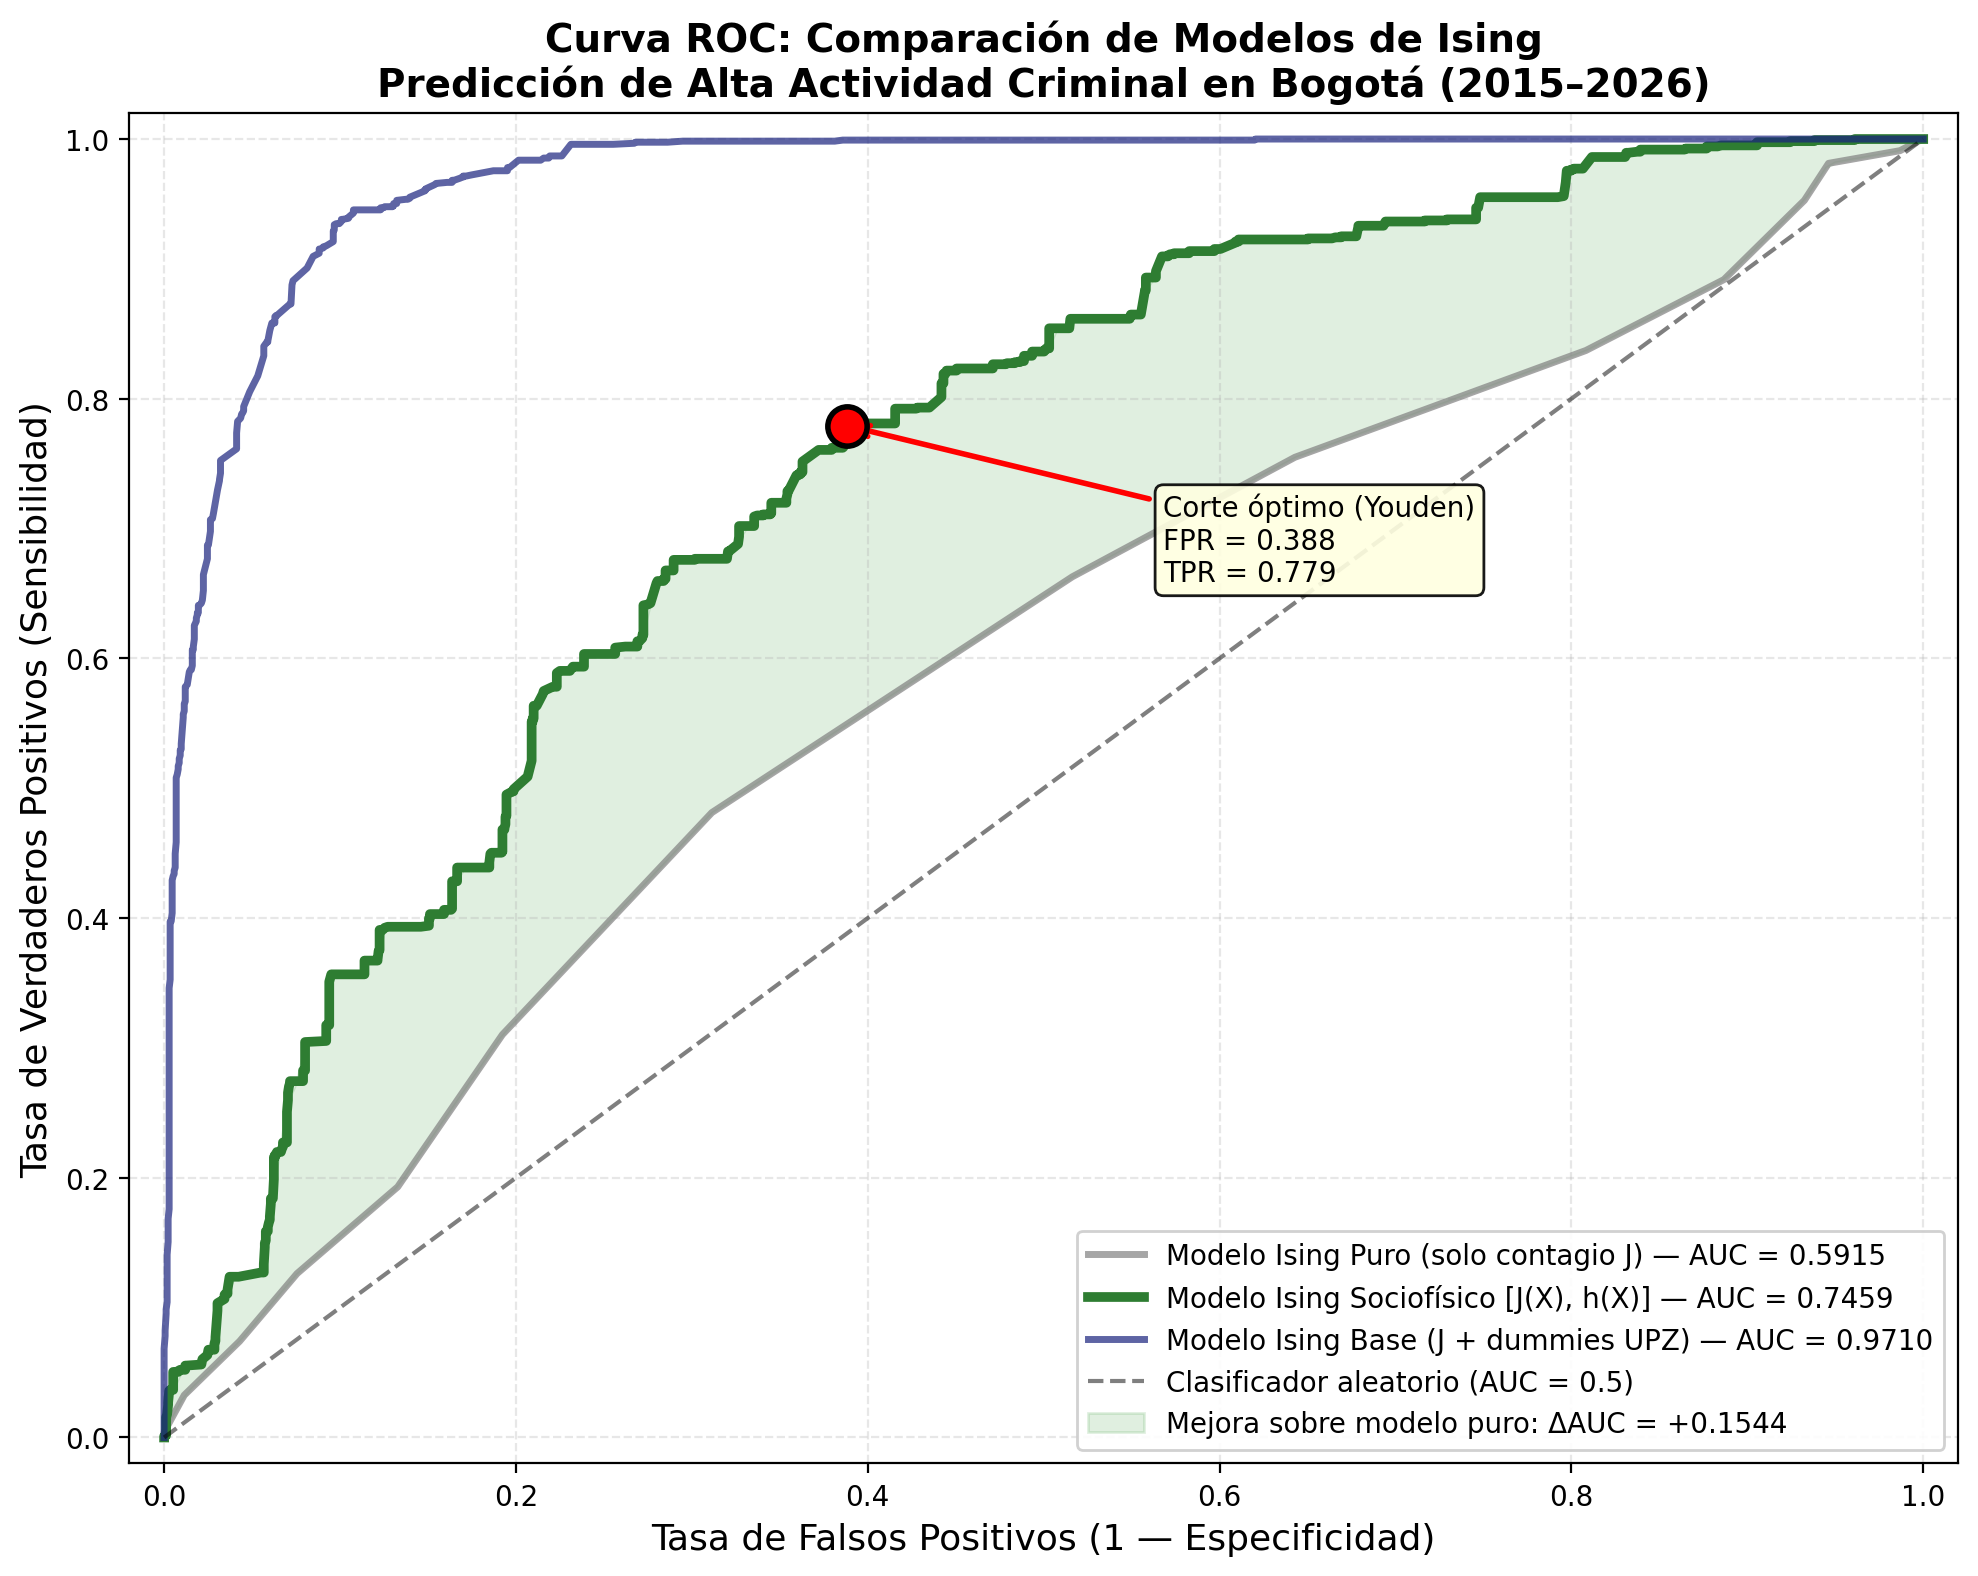
\includegraphics[width=0.88\textwidth]{graficas/fig1_curva_roc.png}
\caption{Curva ROC comparativa de los tres modelos de Ising. La línea diagonal representa el clasificador aleatorio (AUC = 0.5). El punto rojo indica el corte óptimo de Youden para el modelo sociofísico. El área sombreada en verde representa la mejora del modelo sociofísico sobre el modelo puro de contagio.}
\label{fig:roc}
\end{figure}

\subsection{Mapa de Campos Locales $h_i$}

La Figura~\ref{fig:mapa_h} presenta la distribución espacial de los campos locales $h_i$ estimados por el modelo base. Estos coeficientes capturan la vulnerabilidad criminal intrínseca de cada UPZ, es decir, la propensión a presentar alta actividad criminal que no es explicada por el contagio de vecinos. Las UPZs en tonos rojos presentan mayor vulnerabilidad ($h_i > 0$); las azules, menor ($h_i < 0$). Se identifican clusters de alta criminalidad en las zonas sur (Localidad de Ciudad Bolívar, Usme) y noroccidental (Localidad de Suba, Engativá) de la ciudad. Las UPZs con valores extremos ($|h_i| > 3.5$) están etiquetadas con su nombre.

\begin{figure}[H]
\centering
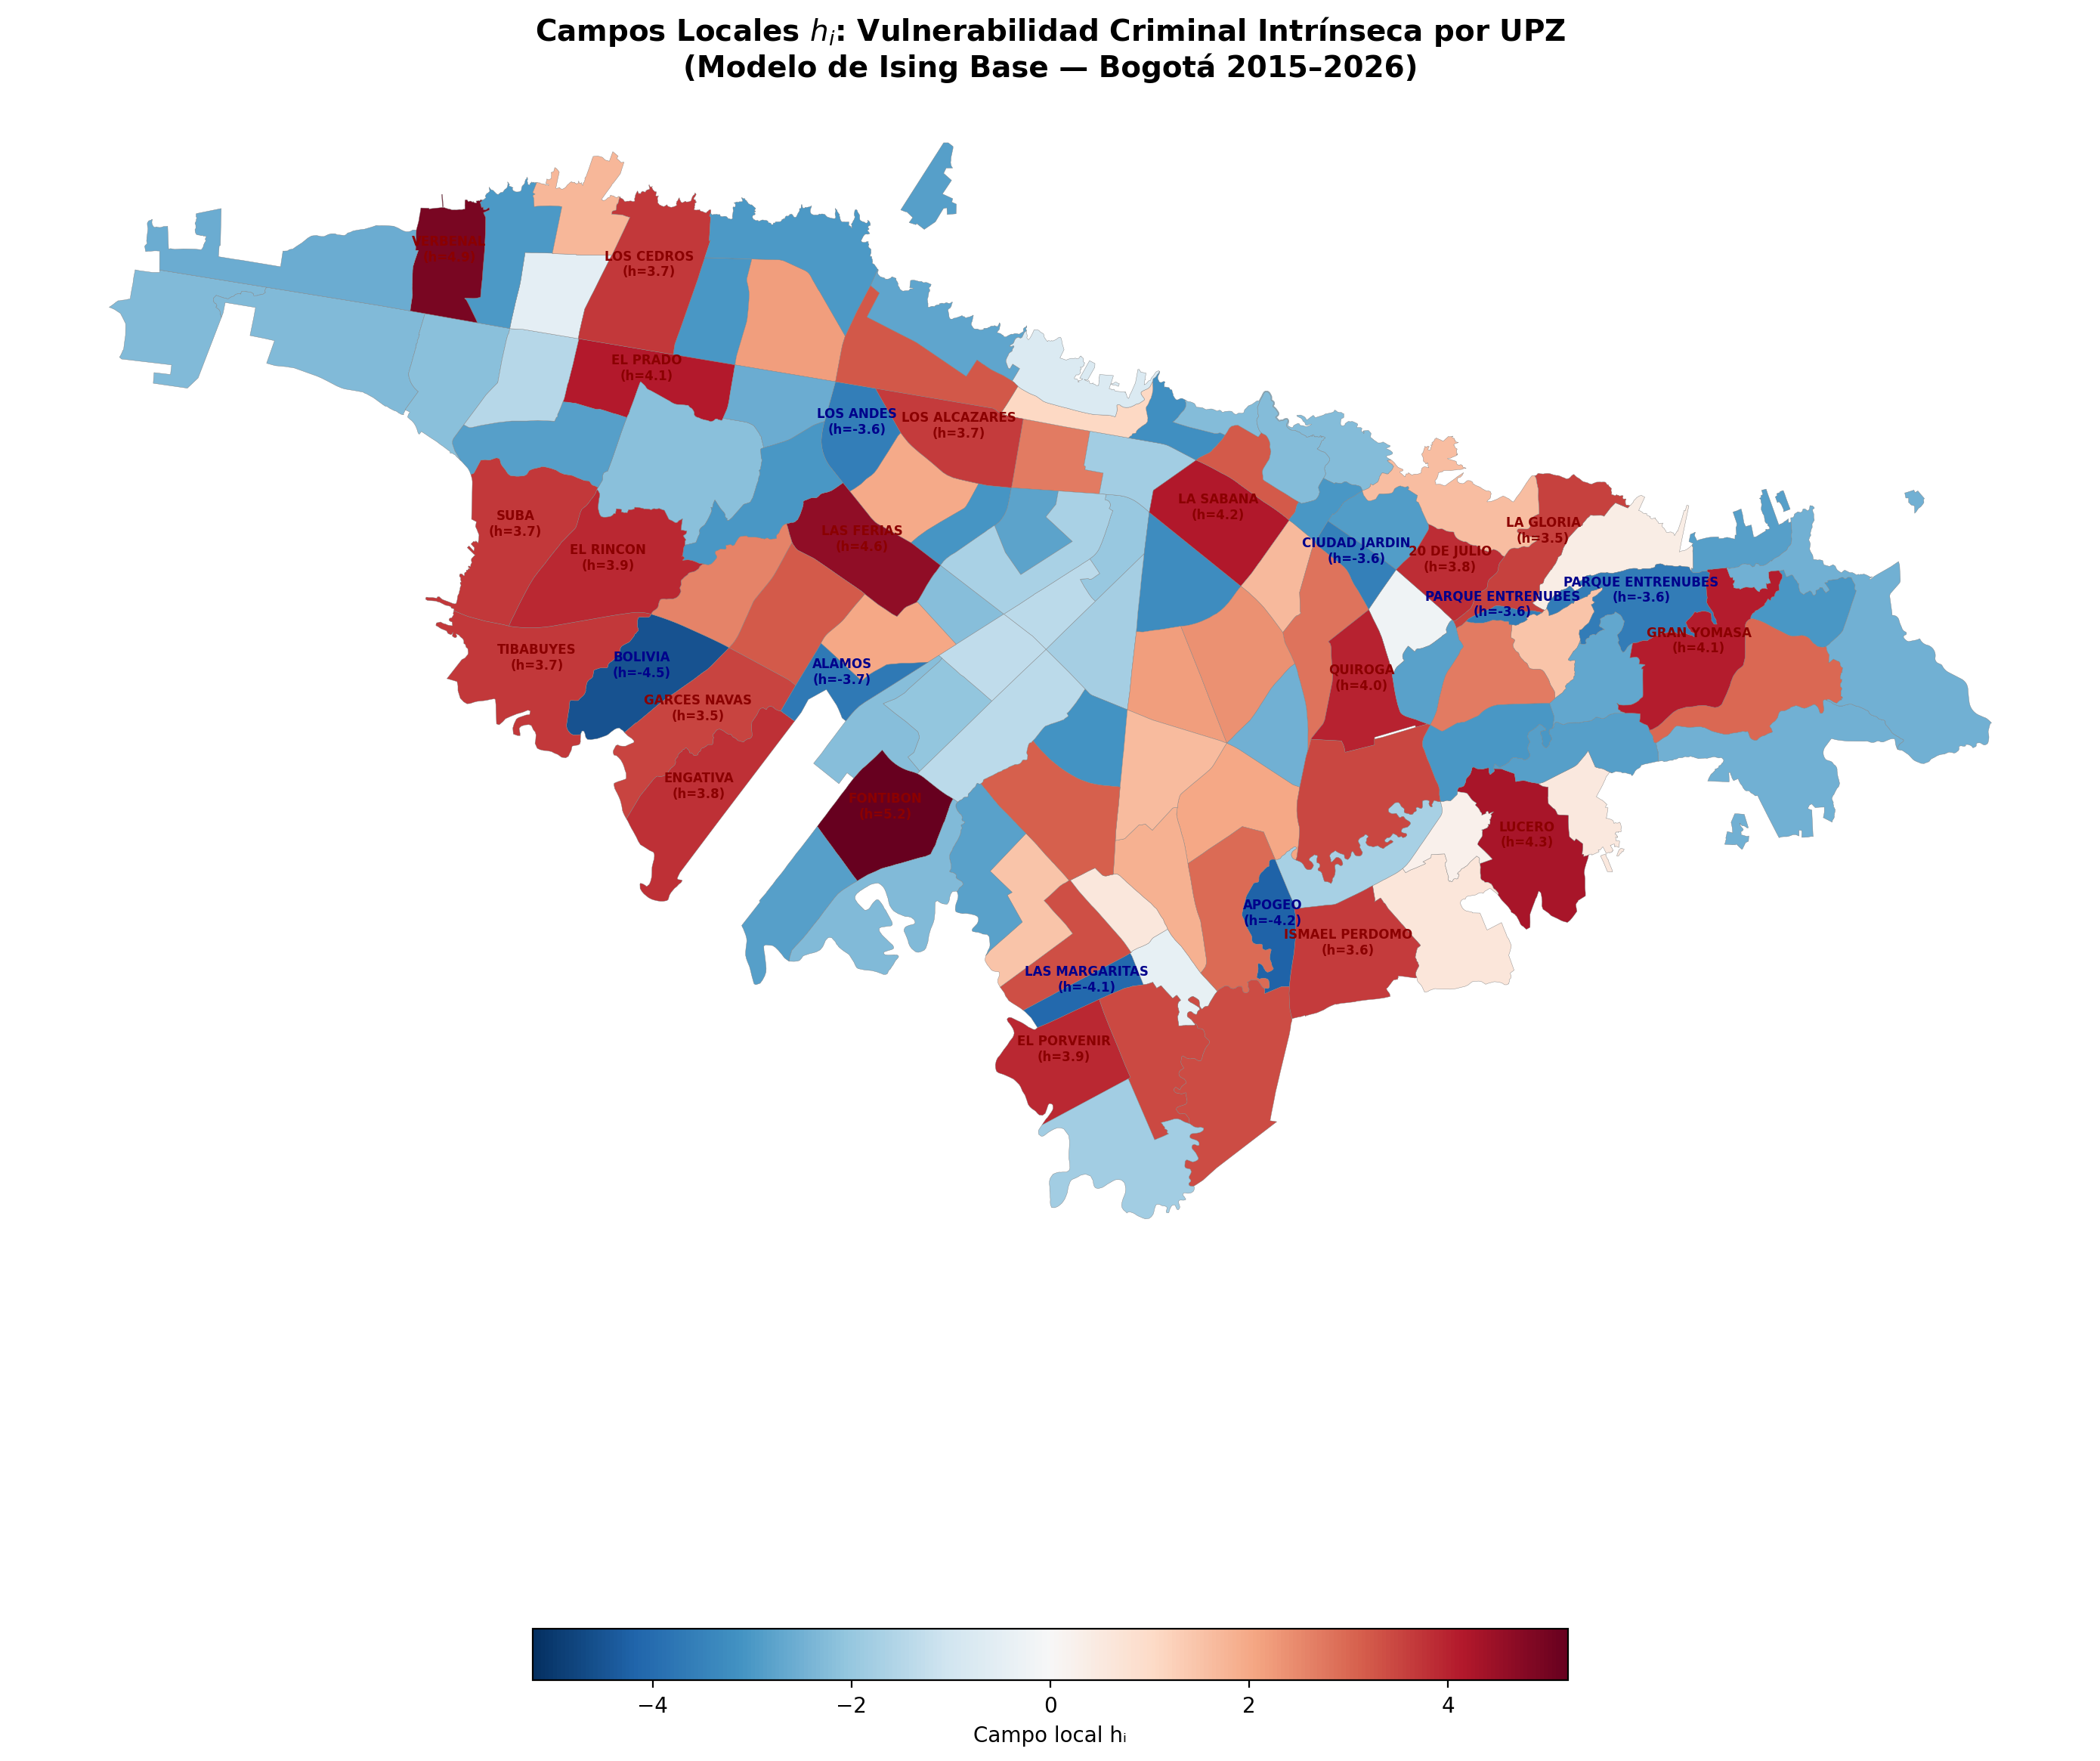
\includegraphics[width=0.88\textwidth]{graficas/fig2_mapa_campos_locales.png}
\caption{Campos locales $h_i$: vulnerabilidad criminal intrínseca por UPZ estimada mediante el modelo de Ising base con regularización L2. La escala de color es simétrica (RdBu\_r) centrada en cero.}
\label{fig:mapa_h}
\end{figure}

\subsection{Coeficientes del Modelo Sociofísico}

\begin{table}[H]
\centering
\caption{Coeficientes del modelo de Ising sociofísico}
\label{tab:coeficientes}
\begin{tabular}{@{}lrl@{}}
\toprule
\textbf{Variable} & \textbf{Coeficiente} & \textbf{Interpretación} \\
\midrule
\multicolumn{3}{c}{\textit{Efectos sobre el CONTAGIO ($J$)}} \\
\midrule
deserción\_promedio & $-0.085^{**}$ & BLOQUEA el contagio \\
n\_cais & $+0.116^{***}$ & AMPLIFICA el contagio \\
estrato\_medio & $+0.039^{*}$ & AMPLIFICA el contagio \\
densidad\_cais & $+0.048^{*}$ & AMPLIFICA el contagio \\
\midrule
\multicolumn{3}{c}{\textit{Efectos sobre el CAMPO LOCAL ($h$)}} \\
\midrule
deserción\_promedio & $+0.199^{***}$ & AUMENTA crimen local \\
estrato\_medio & $-0.393^{***}$ & REDUCE crimen local \\
n\_cais & $+0.088^{**}$ & AUMENTA crimen local \\
densidad\_cais & $-0.023^{*}$ & REDUCE crimen local \\
\bottomrule
\end{tabular}
\end{table}

Los coeficientes de la Tabla~\ref{tab:coeficientes} revelan patrones significativos. La deserción escolar promedio presenta el fenómeno más notable: bloquea el contagio espacial ($\beta = -0.085$) pero simultáneamente aumenta la propensión criminal local ($\alpha = +0.199$). Esto sugiere la formación de ``islas'' de crimen autónomo en zonas con alta deserción. El estrato socioeconómico medio muestra el patrón opuesto: amplifica el contagio ($\beta = +0.039$) pero reduce el crimen local ($\alpha = -0.393$). Los CAIs presentan signos positivos tanto en $J$ como en $h$, reflejando endogeneidad en su ubicación.

\subsection{Evolución del Poder Explicativo}

La Figura~\ref{fig:r2} documenta la evolución del poder explicativo ($R^2$) de los campos locales $h_i$ al incorporar progresivamente fuentes de datos más ricas. Partiendo de proxies geométricos (área, perímetro, compacidad) que explican apenas el 9.4\% de la varianza, la incorporación de tasas de cobertura educativa eleva el $R^2$ al 22.4\%. Finalmente, la integración de datos abiertos completos (estratificación, deserción escolar, CAIs) permite alcanzar un \textbf{$R^2 = 92.5\%$}. Las variables educativas son 2.6 veces más explicativas que los proxies geométricos iniciales.

El panel derecho muestra las correlaciones de Pearson de cada covariable con $h_i$. La deserción escolar (en sus tres métricas: mínimo, máximo y promedio) es consistentemente la variable más correlacionada ($r \approx 0.45-0.54$), seguida por el área de la UPZ ($r = 0.42$).

\begin{figure}[H]
\centering
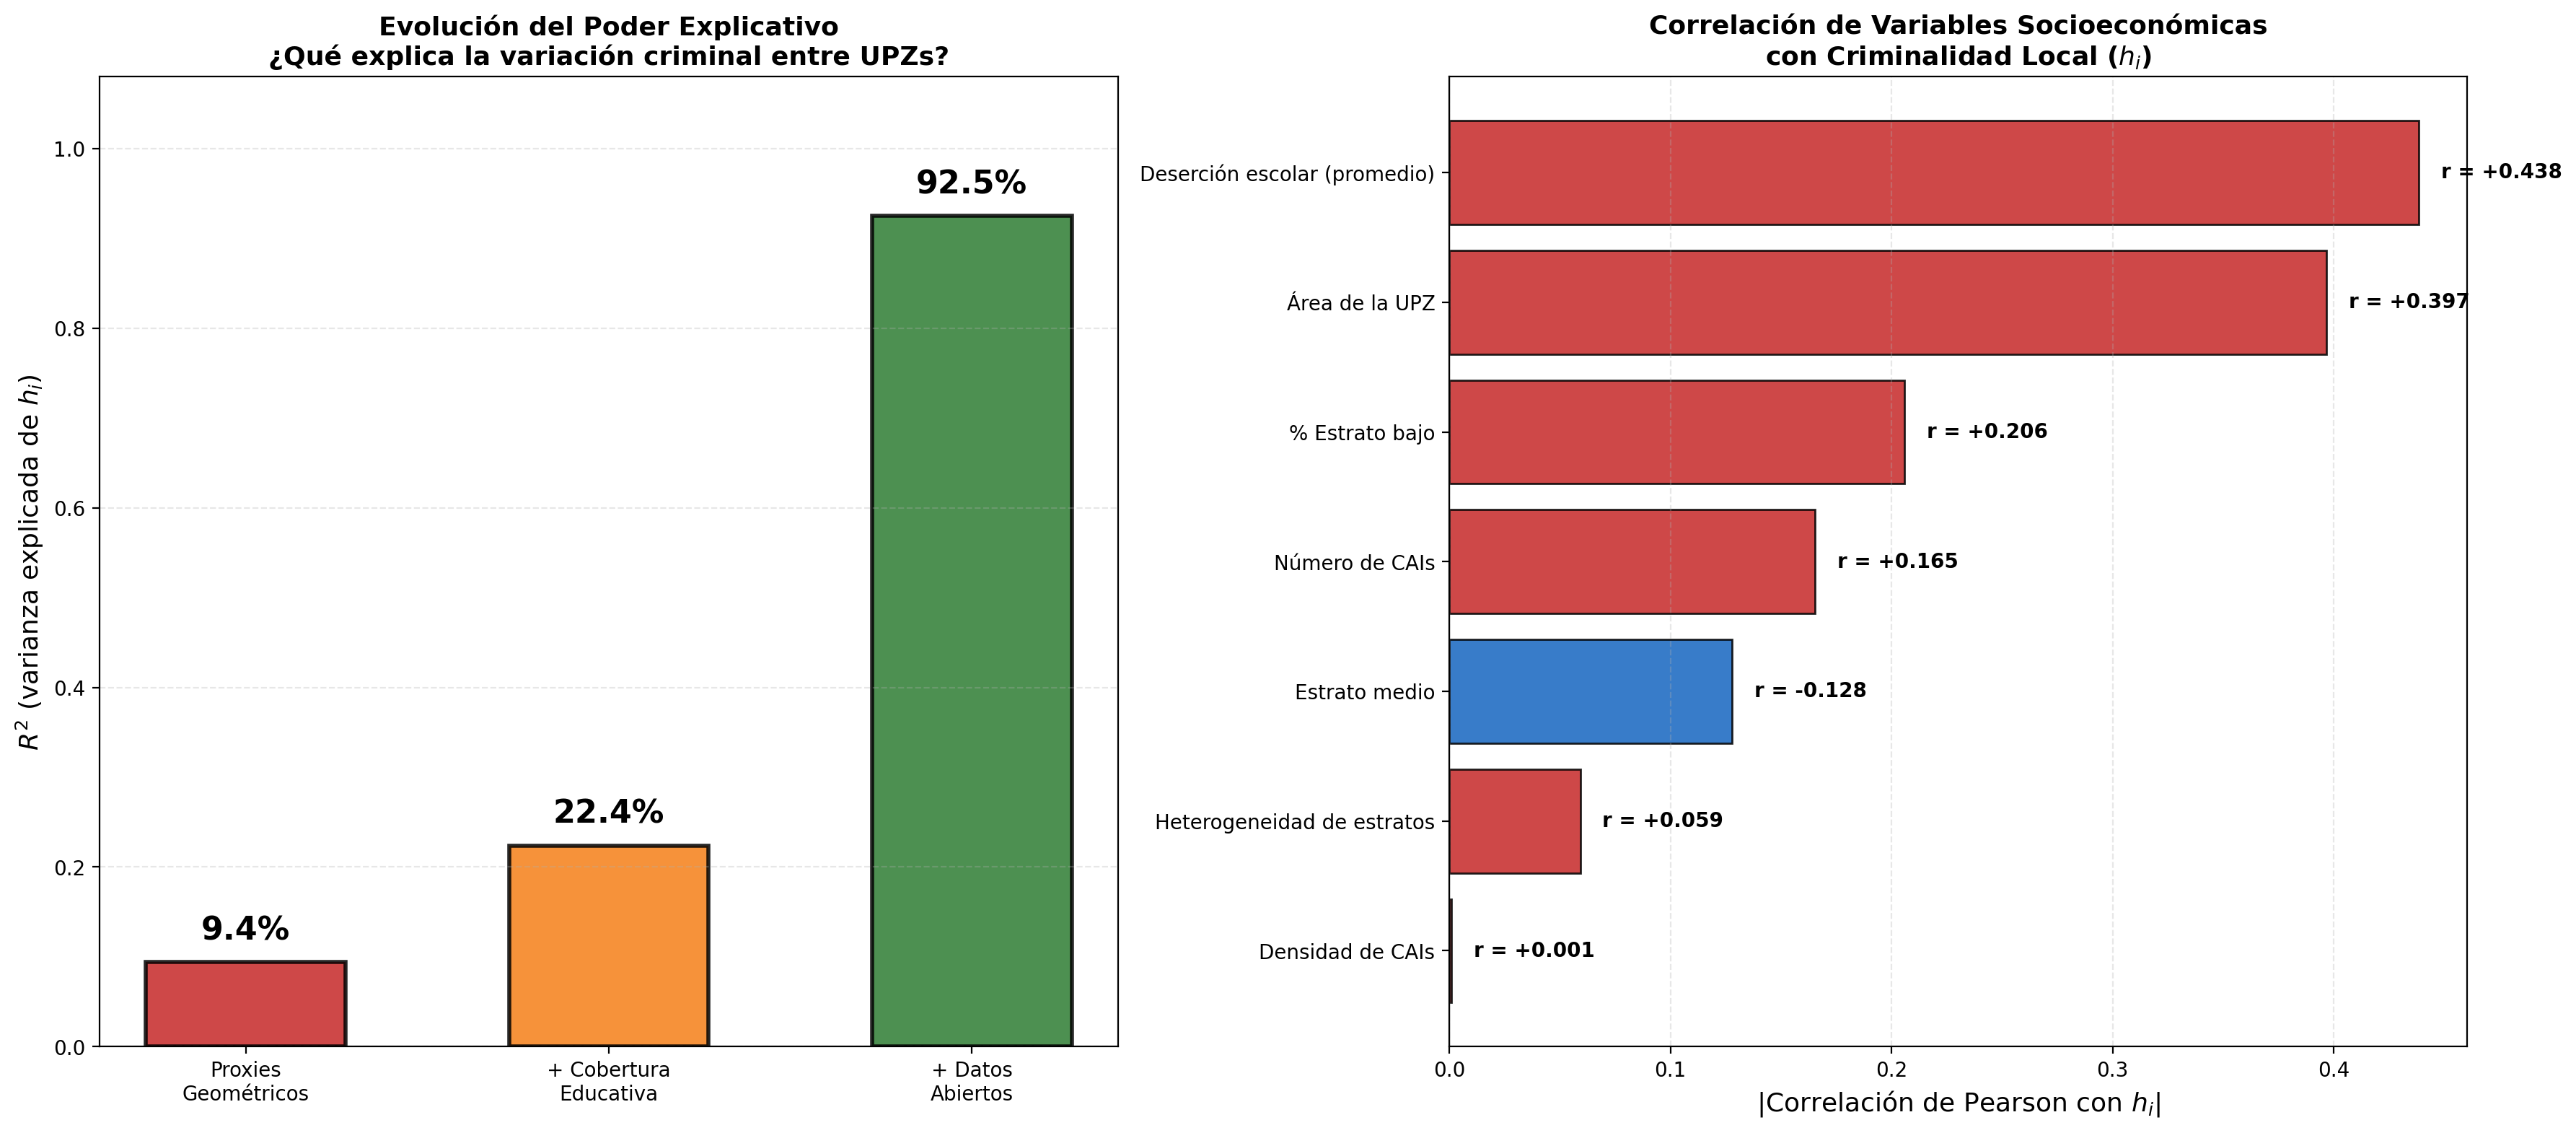
\includegraphics[width=1.0\textwidth]{graficas/fig4_evolucion_R2_correlaciones.png}
\caption{Izquierda: evolución del poder explicativo ($R^2$) de $h_i$ en tres etapas de incorporación de datos. Derecha: correlaciones de Pearson de cada covariable socioeconómica con la criminalidad local ($h_i$). Las barras rojas indican correlación positiva; las azules, negativa.}
\label{fig:r2}
\end{figure}

\subsection{Fase Termodinámica}

Mediante simulación Monte Carlo del modelo de Ising con $J=0.4336$ y los $h_i$ estimados, barriendo temperaturas $T \in [0.5, 8.0]$ y minimizando el error cuadrático ponderado entre observables simulados y reales, se obtiene:
\begin{itemize}
    \item $T_{\text{eff}} = 1.29$ (temperatura efectiva que mejor ajusta los observables)
    \item $T_{\text{crit}} = 0.89$ (temperatura de máxima susceptibilidad)
    \item \textbf{Fase: DESORDENADA} ($T_{\text{eff}} > T_{\text{crit}}$)
\end{itemize}

En fase desordenada, las fluctuaciones aleatorias dominan sobre el orden magnético. Los hotspots criminales son efímeros —aparecen y desaparecen rápidamente— y el sistema es altamente sensible a perturbaciones externas pero no responde de forma colectiva coordinada.

\subsection{Top 10 UPZs con Mayor Criminalidad}

\begin{table}[H]
\centering
\caption{UPZs con mayor $h_i$ (vulnerabilidad criminal intrínseca)}
\label{tab:top10}
\begin{tabular}{@{}rlccc@{}}
\toprule
\textbf{\#} & \textbf{UPZ} & \textbf{$h_i$} & \textbf{Deserción (\%)} & \textbf{Estrato} \\
\midrule
1 & FONTIBON & +5.21 & 4.4 & 2.8 \\
2 & VERBENAL & +4.93 & 3.9 & 3.0 \\
3 & LAS FERIAS & +4.61 & 1.9 & 2.6 \\
4 & LUCERO & +4.31 & 3.8 & 3.0 \\
5 & LA SABANA & +4.16 & 3.9 & 3.2 \\
6 & EL PRADO & +4.14 & 2.9 & 2.5 \\
7 & GRAN YOMASA & +4.09 & 2.1 & 3.0 \\
8 & QUIROGA & +3.99 & 4.5 & 1.0 \\
9 & EL PORVENIR & +3.93 & 2.1 & 2.1 \\
10 & EL RINCON & +3.92 & 3.2 & 2.0 \\
\bottomrule
\end{tabular}
\end{table}

La Tabla~\ref{tab:top10} identifica las diez UPZs con mayor vulnerabilidad criminal intrínseca. FONTIBON y VERBENAL lideran con $h_i > 4.9$, combinando deserción elevada y estrato bajo. QUIROGA destaca con el estrato más bajo (1.0) y la segunda tasa de deserción más alta (4.5\%), representando un caso extremo de vulnerabilidad múltiple.

% ============================================================================
% 7. DISCUSIÓN
% ============================================================================
\section{Discusión}

\subsection{Interpretación de los Hallazgos}

\textbf{1. La deserción escolar es el predictor más robusto de criminalidad.} Con $r = 0.54$ y coeficientes significativos tanto en $J$ como en $h$, la deserción escolar emerge como el factor estructural más relevante. El signo negativo en $J$ sugiere que la deserción crea ``islas'' de crimen autónomo: zonas donde el crimen es endémico pero no se propaga fácilmente a vecinos. Este hallazgo tiene implicaciones directas para la política educativa como herramienta de prevención criminal.

\textbf{2. El estrato socioeconómico tiene efectos opuestos sobre $J$ y $h$.} Zonas de estrato alto reducen el crimen local ($\alpha = -0.393$) pero amplifican el contagio ($\beta = +0.039$). Esto podría explicarse por la mayor movilidad y flujo de personas en zonas acomodadas, que facilitan la propagación del crimen desde zonas vecinas mientras mantienen baja la criminalidad endógena.

\textbf{3. Los CAIs son reactivos, no preventivos.} La correlación positiva entre número de CAIs y criminalidad local ($\alpha = +0.088$) refleja endogeneidad en su ubicación: los comandos policiales se instalan donde ya existe el problema, no necesariamente lo reducen. Sin embargo, la densidad de CAIs muestra un efecto reductor marginal ($\alpha = -0.023$), sugiriendo que la concentración de presencia policial puede tener efectos disuasivos.

\textbf{4. El sistema está en fase desordenada.} Con $T_{\text{eff}} = 1.29 > T_{\text{crit}} = 0.89$, el ruido domina sobre el orden magnético. Esto implica que: (a) los hotspots criminales son inherentemente efímeros, (b) intervenciones puntuales pueden tener efectos impredecibles, y (c) se requieren estrategias sostenidas y sistemáticas más que operativos quirúrgicos aislados.

\subsection{Limitaciones}
\begin{enumerate}[label=\alph*)]
    \item \textbf{Endogeneidad}: Variables como el número de CAIs son endógenas (se instalan donde hay crimen), lo que limita la interpretación causal de los coeficientes.
    \item \textbf{Datos faltantes}: Solo 77 de 113 UPZs tienen datos completos de estratificación; las 36 restantes requieren imputación o exclusión.
    \item \textbf{Agregación temporal}: El modelo utiliza datos mensuales; podrían existir dinámicas semanales o diarias no capturadas (efectos de fin de semana, quincena, etc.).
    \item \textbf{Causalidad}: Las correlaciones reportadas no implican necesariamente relaciones causales; se requieren diseños cuasi-experimentales (diferencias en diferencias, regresión discontinua) para establecer causalidad.
\end{enumerate}

\subsection{Implicaciones para Política Pública}
\begin{enumerate}[label=\alph*)]
    \item \textbf{Intervención educativa prioritaria}: Programas de retención escolar focalizados en las 10 UPZs con mayor $h_i$, con especial atención a hombres en grados 10 y 11.
    \item \textbf{Estrategia territorial diferenciada}: UPZs grandes (alto Shape\_Area) requieren estrategias de escala y coordinación intermunicipal; UPZs pequeñas permiten intervenciones focalizadas de alto impacto.
    \item \textbf{Revisión de la política de CAIs}: Evaluar la efectividad real de los comandos existentes mediante diseños experimentales; considerar redistribución hacia zonas con potencial preventivo en lugar de meramente reactivo.
    \item \textbf{Monitoreo de temperatura efectiva}: Implementar un sistema de alerta temprana que estime $T_{\text{eff}}$ en tiempo real para identificar ventanas de alta susceptibilidad donde las intervenciones tienen máximo impacto.
\end{enumerate}

% ============================================================================
% 8. CONCLUSIONES
% ============================================================================
\section{Conclusiones}

Este proyecto demuestra que el modelo de Ising, enriquecido con datos socioeconómicos, constituye una herramienta metodológicamente rigurosa y empíricamente validada para entender y predecir la criminalidad urbana. Las principales contribuciones son:

\begin{enumerate}[label=\alph*)]
    \item \textbf{Validación empírica del contagio criminal}: El parámetro $J = 0.4336$ es estadísticamente significativo, confirmando que el crimen se propaga entre UPZs vecinas, aunque el efecto es moderado comparado con los factores locales. La correlación espacial es significativa ($p < 0.001$) según pruebas de permutación.
    
    \item \textbf{Identificación de factores estructurales}: El 92.5\% de la variación en $h_i$ entre UPZs puede explicarse mediante variables observables de fuentes abiertas, siendo la deserción escolar el predictor más robusto y consistente.
    
    \item \textbf{Marco interpretable y accionable}: El modelo sociofísico descompone el efecto de cada variable sobre el contagio espacial ($J$) y sobre la propensión local ($h$), proporcionando una lectura dual que enriquece el análisis criminológico tradicional y permite diseñar intervenciones diferenciadas.
    
    \item \textbf{Herramienta de simulación para política pública}: El modelo calibrado permite simular escenarios de intervención (reducir deserción, modificar presencia policial) y estimar su impacto esperado antes de la implementación, reduciendo la incertidumbre en la asignación de recursos públicos.
\end{enumerate}

Trabajo futuro incluye: (i) incorporar fuentes adicionales de datos abiertos (alumbrado público, consumo de sustancias psicoactivas, violencia intrafamiliar, movilidad en TransMilenio), (ii) explorar modelos con $J$ dependiente del tiempo mediante ventanas móviles, (iii) validar las predicciones con datos de 2024-2025 no utilizados durante el entrenamiento, y (iv) extender la metodología a otras ciudades colombianas para evaluar su generalizabilidad.

\newpage
\nocite{*}
\printbibliography[title={Bibliografía}]

% ============================================================================
% APÉNDICE
% ============================================================================

\newpage
\appendix
\section{Fórmulas del Modelo}

\textbf{Probabilidad de activación}:
\begin{equation}
P(s_i=+1) = \frac{1}{1 + \exp\left(-\left[J_i \sum_{j \in \partial i} s_j + h_i\right]\right)}
\end{equation}

\textbf{Función de verosimilitud} (para estimación por máxima verosimilitud):
\begin{equation}
\mathcal{L}(J, \{h_i\}) = \prod_{t} \prod_{i} P(s_i(t+1) \mid \mathbf{s}(t))^{y_{it}} (1 - P(s_i(t+1) \mid \mathbf{s}(t)))^{1-y_{it}}
\end{equation}

\textbf{Algoritmo de Metropolis} (para simulación termodinámica):
\begin{enumerate}
    \item Seleccionar UPZ aleatoria $i$
    \item Calcular cambio de energía: $\Delta E = 2s_i\left(J\sum_{j \in \partial i} s_j + h_i\right)$
    \item Si $\Delta E \leq 0$, aceptar el cambio de estado
    \item Si $\Delta E > 0$, aceptar con probabilidad $\exp(-\Delta E / T)$
\end{enumerate}

\section{Validación con Permutaciones}

Para verificar la significancia estadística de la correlación espacial observada, se realizaron 200 permutaciones de los espines. En cada permutación, se barajaron aleatoriamente las etiquetas de UPZ dentro de cada mes, destruyendo la estructura espacial pero manteniendo la distribución marginal de estados. Resultados:
\begin{itemize}
    \item Correlación espacial: $C_{\text{obs}} = 0.1210$ vs $E[C_{\text{null}}] = 0.1143$ con $p < 0.001$ (estadísticamente significativa)
    \item Susceptibilidad: $\chi_{\text{obs}} = 2.78$ vs $E[\chi_{\text{null}}] = 28.96$ con $p = 1.000$ (no significativa)
\end{itemize}

La correlación espacial observada es significativamente mayor que la esperada por azar, confirmando que el crimen forma clusters geográficos reales. La susceptibilidad, por el contrario, no difiere de la distribución nula, indicando que la ciudad no responde de forma colectiva coordinada a shocks externos.

\section{Especificaciones Técnicas del Pipeline}

\begin{table}[H]
\centering
\caption{Especificaciones del entorno computacional}
\label{tab:specs}
\begin{tabular}{@{}ll@{}}
\toprule
\textbf{Componente} & \textbf{Especificación} \\
\midrule
Lenguaje & Python 3.12 \\
IDE & Jupyter Notebook / CoCalc \\
Sistema operativo & Linux (CoCalc) / Windows 11 \\
Memoria utilizada & $\sim$4 GB \\
Tiempo de ejecución total & $\sim$15-20 minutos \\
\bottomrule
\end{tabular}
\end{table}

\end{document}